\documentclass[11pt]{article}
\usepackage{amsmath, amssymb}
\usepackage[margin=1in]{geometry}
\usepackage{enumitem}
\usepackage{graphicx}
\setlength{\parindent}{0pt}
\setlength{\parskip}{6pt}

\title{Live test on a real phone\\[2pt]
\large streaming phone sensors with phyphox and running our maths in real time
(Synheart Kinematics)}
\date{}

\begin{document}
\maketitle

Short note on the live demo: instead of only testing on saved datasets, I streamed the
motion sensor off my own phone over Wi-Fi and ran the Activity-State / Movement-Regularity
maths on it \emph{live}.

\section{Setup}
\begin{itemize}[noitemsep]
  \item Phone and laptop on the same Wi-Fi. The phone runs \textbf{phyphox}
        (\textit{Acceleration with g}) with \textbf{Remote Access} on --- this makes the
        phone serve its sensor data over a small web address, e.g.\ \texttt{http://<ip>:8080}.
  \item The laptop asks the phone for new samples every $0.1$\,s (the phyphox
        \texttt{/get} endpoint), keeps a \textbf{2-second sliding window}, and runs the rule.
  \item No trained model and no internet --- our Activity State is a deterministic
        threshold rule, so the laptop just computes it directly.
\end{itemize}

\section{What it computes (live, every $\sim\!0.4$\,s)}
From the three sensor axes $x,y,z$:
\[
  |a|=\sqrt{x^2+y^2+z^2}\quad(\text{strength of acceleration}),\qquad
  \texttt{movement}=\operatorname{std}\big(|a|\big)\ \text{over the window}.
\]
\begin{itemize}[noitemsep]
  \item \textbf{$|a|$} --- at rest this is just gravity ($\approx 9.8$); motion adds to it.
        Rotating the phone changes the axes but \emph{not} $|a|$ (same length), so it is
        orientation-proof.
  \item \textbf{movement} --- how much $|a|$ wobbles over $2$\,s $=$ how much the person is
        moving. This single number drives the verdict.
  \item \textbf{Activity State} --- a plain rule: $\texttt{movement}<1.2\Rightarrow$ still,
        $1.2$--$4\Rightarrow$ walking, $>4\Rightarrow$ running/vigorous.
  \item \textbf{Movement Regularity} --- whether the wobble repeats (autocorrelation):
        \emph{calm} (still), \emph{rhythmic} (steady walk/run), \emph{erratic} (jerky).
\end{itemize}

\section{What I observed}
The verdict tracked what I actually did, with clean transitions (Fig.~\ref{fig:live}):
\begin{center}
\begin{tabular}{lccl}
what I did & movement (m/s$^2$) & $|a|$ & verdict\\ \hline
held still      & $0.01$--$0.02$ & $\approx 9.86$ & STILL (calm)\\
walked          & $1.5$--$3.6$   & $10$--$11$     & WALKING (rhythmic)\\
ran / shook     & $9$--$14$      & $14$--$20$     & RUNNING/VIGOROUS (rhythmic)\\
stopped         & $\to 0.01$     & $\approx 9.86$ & STILL (calm)\\
\end{tabular}
\end{center}

\begin{figure}[h]
\centering
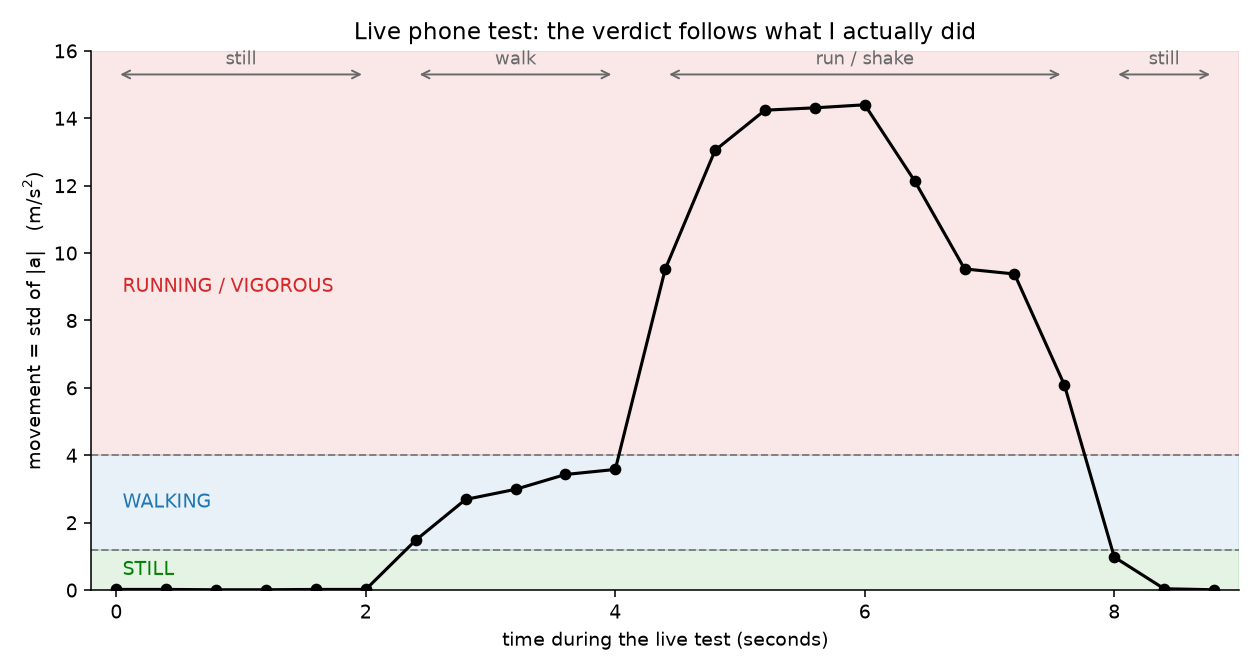
\includegraphics[width=0.85\textwidth]{figs/fig_live.png}
\caption{Real values captured during the live test. \texttt{movement} (one number from
$|a|$) rises and falls exactly with what I did; the dashed lines are the still/walking/running
thresholds.}
\label{fig:live}
\end{figure}

\textbf{The orientation-proof moment.} Holding the phone still and rotating it to a different
orientation: the per-axis numbers swing (gravity moves between $x$, $y$, $z$), but $|a|$,
\texttt{movement} and the verdict stay put. Orientation changed completely; the activity
reading did not --- because $\lVert R\mathbf a\rVert=\lVert\mathbf a\rVert$.

\section{What this shows}
\begin{itemize}[noitemsep]
  \item Both deliverables --- \textbf{Activity State} and \textbf{Movement Regularity} ---
        run \textbf{live, in real time, on a brand-new device} (a phone, not the training
        data), straight from the raw sensor.
  \item It stays \textbf{orientation-proof} on real hardware, not just on paper.
  \item No sitting/standing/lying: that is posture, which needs gravity \emph{direction}
        (orientation-dependent) and belongs to the separate Postural-State task --- by design.
\end{itemize}

This is the real-world face-check on top of the measured results: \textbf{0\% drop under
rotation on UCI-HAR} and \textbf{89\% on unseen people in PAMAP2}. Measured on two datasets,
and now running live on my own phone.

\end{document}
